% !TEX TS-program = xelatex
\documentclass[aspectratio=169]{beamer}

% --- THEME & LAYOUT ---
\usetheme[numbering=fraction,progressbar=head]{metropolis}
\setbeamersize{text margin left=8mm,text margin right=8mm}

% --- CUSTOM FOOTER WITH TLP MARKING ---
\setbeamertemplate{frame footer}{\textbf{TLP:CLEAR} -- Information may be shared freely without restriction.}
\setbeamercolor{frame footer}{fg=cyber-accent}

\usepackage{amsmath}

% --- FONTS (XeLaTeX) ---
\usepackage{fontspec}
\setsansfont[
  Ligatures=TeX, Scale=1.02,
  BoldFont = {IBM Plex Sans Bold},
  ItalicFont = {IBM Plex Sans Italic}
]{IBM Plex Sans}
\setmonofont{IBM Plex Mono}

% --- ICONS ---
\usepackage{fontawesome5}

% --- COLORS (cyber palette) ---
\definecolor{cyber-bg}{HTML}{0B0F14}
\definecolor{cyber-ink}{HTML}{E6EEF5}
\definecolor{cyber-accent}{HTML}{217EAA}
\definecolor{cyber-mid}{HTML}{7D9CB7}
\definecolor{cyber-soft}{HTML}{8CA4AC}
\setbeamercolor{normal text}{fg=cyber-ink,bg=cyber-bg}
\setbeamercolor{frametitle}{fg=cyber-ink,bg=cyber-bg}
\setbeamercolor{progress bar}{fg=cyber-accent,bg=cyber-soft}
\setbeamercolor{alerted text}{fg=cyber-accent}

% --- LINKS ---
\hypersetup{colorlinks=true, linkcolor=cyber-accent, urlcolor=cyber-accent}

% --- CODE / BOXES ---
\usepackage{listings}
\lstset{
  basicstyle=\ttfamily\footnotesize,
  backgroundcolor=\color{black!5},
  frame=single, rulecolor=\color{cyber-soft},
  keywordstyle=\color{cyber-accent}\bfseries,
  commentstyle=\color{cyber-soft},
  showstringspaces=false
}
\usepackage[most]{tcolorbox}
\tcbset{colback=black!5!cyber-bg, colframe=cyber-soft, coltext=cyber-ink, boxsep=1mm, left=2mm, right=2mm}

% --- PDF TOOLS ---
\usepackage{pdfpages}

% --- GRAPHICS ---
\usepackage{graphicx}

% --- SPEAKER NOTES ---
\usepackage{pgfpages}
% \setbeameroption{hide notes}
% \setbeameroption{show notes}
% \setbeameroption{show only notes}

% --- SPACING IMPROVEMENTS ---
\setbeamertemplate{itemize/enumerate body begin}{\vspace{-0.5ex}}
\setbeamertemplate{itemize/enumerate subbody begin}{\vspace{-0.5ex}}

% --- TITLE INFO ---
\title{\faIcon{shield-alt}\; Range42 -- Status Update}
\subtitle{Open Cyber Range Platform for Collaborative Security Training}
\author{NC3 / Range42 Team}
\date{October 2026}
\institute{\faServer\; Proxmox \quad \faCogs\; Ansible \quad \faProjectDiagram\; Orchestration \quad \faBinoculars\; Telemetry}

\begin{document}

% === TITLE ===
\begin{frame}[plain,noframenumbering]
  \titlepage
  \note[item]{Goal: 20-minute status update on Range42 over the past year.}
  \note[item]{Audience: cybersecurity professionals, government, European ecosystem partners.}
\end{frame}

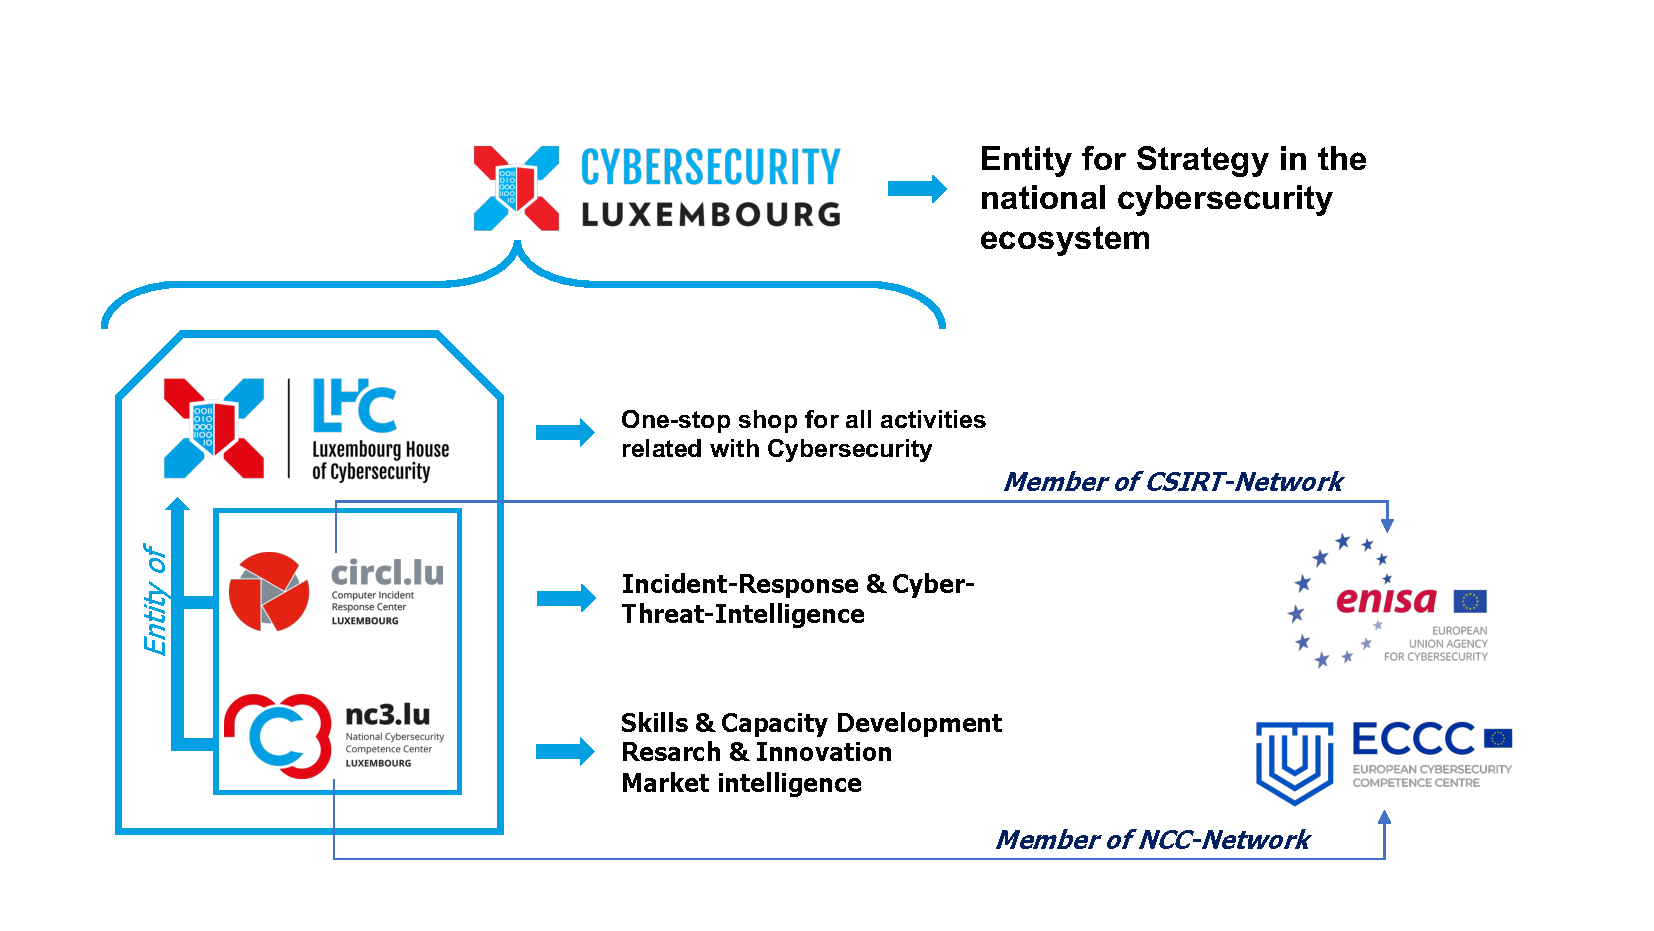
\includepdf[pages={1-2}]{../../pdf_slides/LHC_NC3.pdf}

% === PUBLIC MONEY PUBLIC CODE ===
\begin{frame}{Public Money, Public Code. Let's go all the way, shall we?}
  \begin{columns}[T]
    \column{0.65\textwidth}
    \textbf{Team \& Funding}
    \begin{itemize}
      \item Built and maintained by \textbf{NC3} and \textbf{DIGISQUAD}
      \item Supported by the \textbf{Directorate of Defence}
      \item Public grant for cyber training infrastructure
      \item FOSS model: no licensing \textcolor{green}{\faMoneyBill}, transparent development (GPL-3.0)
    \end{itemize}

    \column{0.3\textwidth}
    \vspace{2mm}
    \begin{figure}
      \centering
      
\includegraphics[width=\textwidth]{../../images/logos/FSFE_Public_Money_Public_Code_logo.pdf}
    \end{figure}
  \end{columns}
  \note[item]{Emphasize public funding = public ownership = public benefit.}
\end{frame}

% === AGENDA ===
\begin{frame}{Agenda}
  \begin{enumerate}
    \item What Range42 is \& why it matters
    \item Progress over the year: what's new
    \item Architecture: two ways in, one engine
    \item Operator CLI, Deployer UI \& content catalog
    \item Exercise tooling around the range
    \item Today vs.\ tomorrow, roadmap
    \item How to get involved
  \end{enumerate}
  \note[item]{No live demo this time: the deployer and CLI are covered through their capabilities.}
\end{frame}

% === WHAT IS RANGE42 ===
\begin{frame}{What is Range42?}
  \begin{itemize}
    \item \textbf{Open cyber range platform} for offensive, defensive, and hybrid training
    \item \textbf{Reproducible Infrastructure-as-Code}: Proxmox, Ansible, Docker
    \item \textbf{One operator workstation}, many Proxmox infrastructures, many lab scenarios each
    \item \textbf{Flexible \& extensible}: network labs, product labs, CVE \& misconfiguration labs, detection workshops
  \end{itemize}
  \begin{tcolorbox}
    \faInfoCircle\; Built to simulate \emph{real-world incidents} safely, with isolation, snapshots, and telemetry.
  \end{tcolorbox}
  \note[item]{Anchor on "safe realism" and extensibility.}
\end{frame}

% === PROGRESS OVER THE YEAR ===
\section{Progress Over the Year}

\begin{frame}[shrink=14]{Progress Over the Year \; \faChartLine}
  \color{cyber-ink}
  \textbf{By the Numbers}
  \begin{itemize}
    \item \alert{2{,}500+ commits} on the main branches of \alert{21 repositories}
    \item \alert{1{,}500+ commits in 2026} across the seven core repositories
    \item Playbooks: 396 \;$\cdot$\; Deployer UI: 377 \;$\cdot$\; Backend API: 297 \;$\cdot$\; Range42: 220 \;$\cdot$\; Catalog: 173
  \end{itemize}
  \vspace{1mm}
  \textbf{Key Milestones}
  \begin{itemize}
    \item \alert{Setup wizard} and \alert{\texttt{range42-context}} CLI + TUI for daily operations
    \item \alert{Proxmox SDN networks} and \alert{Proxmox firewall} wired into every deployment
    \item \alert{Git-backed scenario authoring} in the Deployer UI, on a new \texttt{/v1} API
    \item \alert{Product labs} (MISP, Gitea, Mattermost, Nextcloud, Rocket.Chat, Kunai)
    \item \alert{Public documentation site} and \alert{project website}
  \end{itemize}
  \note[item]{Concrete, measurable progress. Counts are from the main branches as of October 2026.}
\end{frame}

% === CURRENT ACHIEVEMENTS ===
\begin{frame}[shrink=12]{Current Achievements \; \faCheckCircle}
  \color{cyber-ink}
  \textbf{What's Working Today}
  \begin{itemize}
    \item \alert{20 scenarios} in range42-playbooks: network, product, defensive and offensive labs
    \item \alert{16 CVE \& misconfiguration bundles}, from Heartbleed to 2025 sudo and Tomcat CVEs
    \item \textbf{Guided install}: one wizard from preflight checks to a deployed lab
    \item \textbf{Segmented networks}: SDN vnets per subnet, per-network NAT, opt-in firewall arming
    \item \textbf{Visual designer} that saves scenarios as Git revisions and deploys them
    \item \textbf{Integrated monitoring} via Wazuh for telemetry and alerting
  \end{itemize}
  \vspace{2mm}
  \begin{tcolorbox}
    \faLightbulb\; \textbf{Key Milestone}: the CLI and the web UI now converge on the same playbooks and the same Proxmox infrastructure.
  \end{tcolorbox}
  \note[item]{Both operator paths are usable today; pick the one that fits the team.}
\end{frame}

% === COMPETITIVE LANDSCAPE ===
\begin{frame}[shrink=5]{Range42 vs.\ Other Cyber Ranges}
  \begin{table}
    \tiny\color{cyber-ink}
    \begin{tabular}{l|cccc}
      \textbf{Feature} & \textbf{Range42} & \textbf{Commercial SaaS} & \textbf{Cloud Native} & \textbf{Traditional} \\
      \hline
      \alert{Open Architecture} & \checkmark & \texttimes & \texttimes & \texttimes \\
      \alert{IaC/GitOps} & \checkmark & \textasciitilde & \checkmark & \texttimes \\
      Private Deployment & \checkmark & \texttimes & \textasciitilde & \checkmark \\
      Cost Control & \checkmark & \texttimes & \textasciitilde & \checkmark \\
      Full Data Custody & \checkmark & \texttimes & \texttimes & \checkmark \\
      API Orchestration & \checkmark & \checkmark & \checkmark & \texttimes \\
      Rapid Reset/Snapshots & \checkmark & \checkmark & \textasciitilde & \textasciitilde \\
      Custom Scenarios & \checkmark & \texttimes & \textasciitilde & \checkmark \\
      \alert{Visual Lab Designer} & \checkmark & \checkmark & \texttimes & \texttimes \\
    \end{tabular}
  \end{table}
  \vspace{1mm}
  \begin{tcolorbox}
    \faLightbulb\; \textbf{Range42's Edge}: Full control, reproducibility, and cost-effectiveness without vendor lock-in.
  \end{tcolorbox}
  \note[item]{IaC/GitOps is now literal: UI scenarios are saved and published as Git revisions.}
\end{frame}

% === ARCHITECTURE ===
\section{Architecture}

\begin{frame}[squeeze]{Architecture at a Glance}
  \begin{itemize}
    \item \textbf{Hypervisor layer}: Proxmox VMs/LXCs; snapshots; SDN zones and vnets; Proxmox firewall
    \item \textbf{Automation layer}: scenarios $\rightarrow$ bundles $\rightarrow$ catalog roles \& Compose stacks; Proxmox controller role
    \item \textbf{Control plane}: Backend API (FastAPI, \texttt{/v1}) running playbooks via ansible-runner; live events over SSE
    \item \textbf{Access layer}: Kong API gateway for auth, ACLs and rate limiting
    \item \textbf{UX layer}: \texttt{range42-context} CLI + TUI, Deployer UI (visual designer)
    \item \textbf{Observability}: Wazuh for logs/alerts; structured logs with secret redaction
  \end{itemize}
  \note[item]{New this year: SDN + firewall at the hypervisor, the CLI/TUI, the v1 API and SSE events.}
\end{frame}

\begin{frame}{Two Ways In, One Engine \; \faProjectDiagram}
  \begin{columns}[T]
    \column{0.48\textwidth}
    \textbf{\faTerminal\; CLI path}
    \begin{itemize}
      \item \texttt{range42-init.py}: setup wizard
      \item \texttt{range42-context}: workspaces, deploy/undeploy, SSH, credentials
      \item Drives Ansible playbooks directly
      \item For advanced and scripted use
    \end{itemize}

    \column{0.48\textwidth}
    \textbf{\faDesktop\; Web path}
    \begin{itemize}
      \item Deployer UI $\rightarrow$ Kong $\rightarrow$ Backend API
      \item Visual topology, preflight, progress, logs
      \item Backend owns attempts, credentials, recovery
      \item For day-to-day operations
    \end{itemize}
  \end{columns}
  \vspace{3mm}
  \begin{tcolorbox}
    \faInfoCircle\; Both paths run the same \textbf{range42-playbooks} against the same Proxmox infrastructure.
  \end{tcolorbox}
  \note[item]{The web UI adds a visual layer and a managed API on top; it does not replace the CLI.}
\end{frame}

\begin{frame}[shrink=8]{Architecture: Logical Components $\rightarrow$ Repository Mapping}
  \begin{figure}
    \centering
    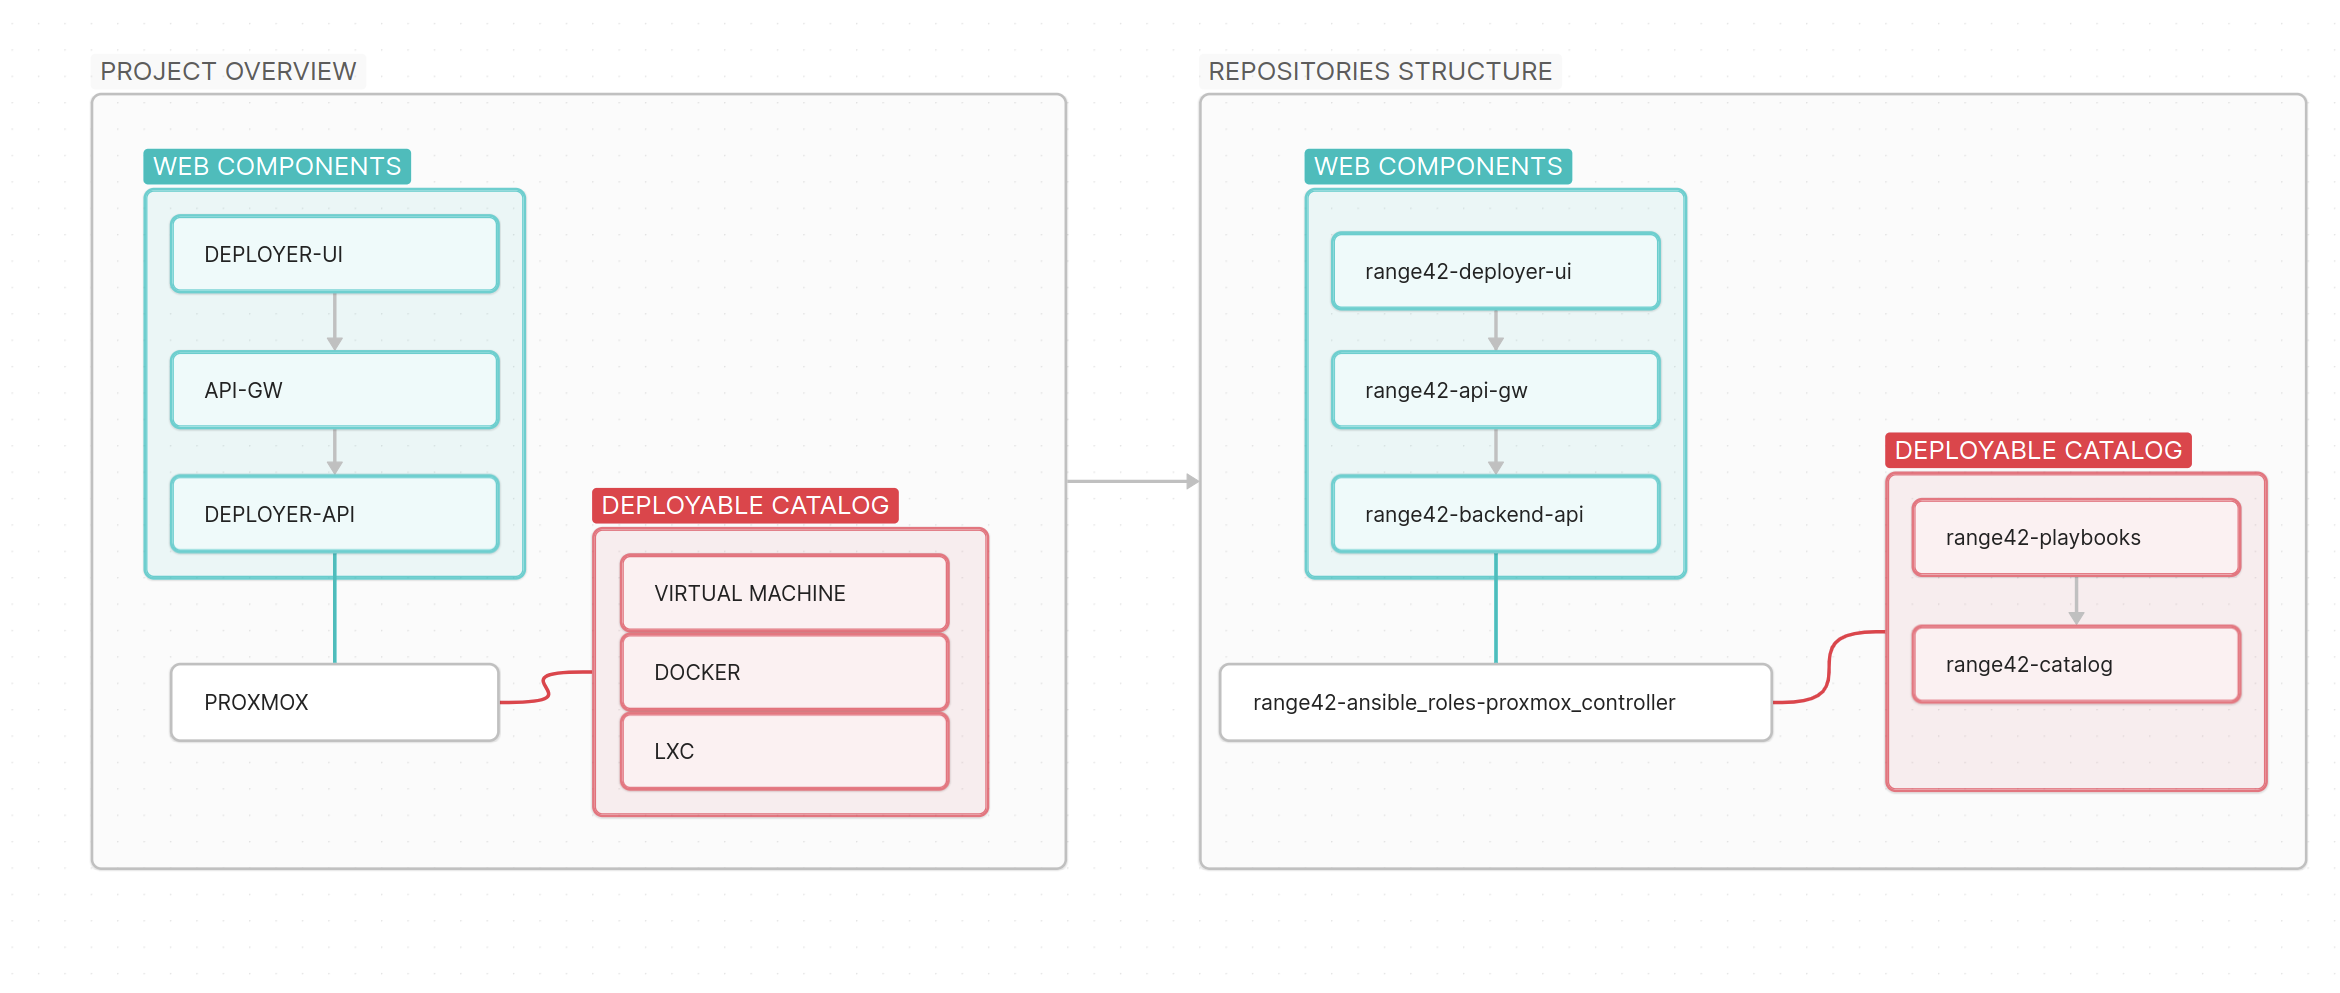
\includegraphics[width=0.95\textwidth]{../../images/diagrams/architecture.png}
  \end{figure}
  \vspace{-3mm}
  \begin{tcolorbox}
    \faInfoCircle\; \textbf{Left}: Logical architecture flow. \textbf{Right}: Actual GitHub repository structure.
  \end{tcolorbox}
  \note[item]{Left side shows logical architecture; right side shows actual GitHub repos.}
\end{frame}

% === OPERATOR CLI ===
\section{Operator Tooling}

\begin{frame}{Setup Wizard \& \texttt{range42-context} \; \faTerminal}
  \begin{columns}[T]
    \column{0.48\textwidth}
    \textbf{\faMagic\; Install}
    \begin{itemize}
      \item Preflight checks, Proxmox connection
      \item SDN networks by default, outbound NAT per network
      \item Optional SSH source whitelist for lab VMs
      \item Optional apt proxy / mirror
    \end{itemize}

    \column{0.48\textwidth}
    \textbf{\faTools\; Operate}
    \begin{itemize}
      \item Switch workspaces, deploy / undeploy
      \item VM lifecycle, snapshots, revert
      \item Egress on/off and firewall arming, by scope
      \item \texttt{catalog-try}: test one catalog element on a disposable VM
      \item \texttt{--tui}: the same gestures in a dashboard
    \end{itemize}
  \end{columns}
  \note[item]{Every gesture takes a scope and a confirmation; the TUI reads its scope from the scenario manifest.}
\end{frame}

% === DEPLOYER UI ===
\begin{frame}{Deployer UI: Visual Lab Designer \; \faDrawPolygon}
  \begin{columns}[T]
    \column{0.48\textwidth}
    \textbf{\faEdit\; Design}
    \begin{itemize}
      \item Canvas: VMs, LXC, SDN networks, multi-NIC guests, notes
      \item Ready-made scenarios from public forks or private repos
      \item Team and user replication into concrete instances
      \item Attach verified catalog bundles to scenario VMs
      \item Save, publish and reopen projects as Git revisions
    \end{itemize}

    \column{0.48\textwidth}
    \textbf{\faPlay\; Deploy}
    \begin{itemize}
      \item Preflight checks before any change
      \item Durable VMID and address reservations
      \item Live progress, logs and events (SSE)
      \item Reviewed runtime network and firewall changes
      \item Import existing guests, snapshot operations
    \end{itemize}
  \end{columns}
  \note[item]{The UI went from drag-and-drop prototype to a Git-backed authoring and deployment tool.}
\end{frame}

% === BACKEND API MATURITY ===
\begin{frame}{Backend API: the \texttt{/v1} Surface \; \faCogs}
  \begin{columns}[T]
    \column{0.48\textwidth}
    \textbf{New API}
    \begin{itemize}
      \item \texttt{/v1}: projects, deployments, catalog, Proxmox hosts
      \item Deployment lifecycle: preflight, attempts, events, teardown
      \item Registered Proxmox hosts: VMs, storage, snapshots
      \item Legacy \texttt{/v0/admin} kept alongside
      \item OpenAPI spec published (121 paths)
    \end{itemize}

    \column{0.48\textwidth}
    \textbf{Hardening}
    \begin{itemize}
      \item \alert{Secret redaction} in logs; workspace secrets shredded after each attempt
      \item \alert{Two-stage Docker image} (Debian bookworm)
      \item \alert{Test suite}: 170+ test modules, CI on every change
      \item Host capacity and deployment budgets reported
    \end{itemize}
  \end{columns}
  \note[item]{Backend owns attempts, credentials and runner recovery; the UI only reviews and observes.}
\end{frame}

% === CONTENT CATALOG ===
\section{Content}

\begin{frame}[shrink=8]{Scenarios \& Catalog \; \faBoxOpen}
  \color{cyber-ink}
  \begin{columns}[T]
    \column{0.48\textwidth}
    \textbf{Scenarios (range42-playbooks)}
    \begin{itemize}
      \item \textbf{Network labs}: blank bases with 2, 4 or 6 subnets
      \item \textbf{Product labs}: MISP, Gitea, Mattermost, Nextcloud, Rocket.Chat
      \item \textbf{Detection workshop}: Kunai
      \item \textbf{Defensive \& offensive}: \texttt{demo\_lab} with Wazuh and vulnerable hosts
    \end{itemize}

    \column{0.48\textwidth}
    \textbf{Building blocks (range42-catalog)}
    \begin{itemize}
      \item \textbf{30 admin roles}: Wazuh, Docker, firewall, Tailscale, users, OAuth2 wiring
      \item \textbf{CVE \& misconfiguration stacks}: OpenSSH, OpenSSL, Apache, Tomcat, PHP, sudo, Vite, pdf.js, Erlang SSH
      \item \textbf{Gamification layer}: themed front-ends (HTML, PHP, Vue)
    \end{itemize}
  \end{columns}
  \vspace{2mm}
  \begin{tcolorbox}
    \faInfoCircle\; Scenarios compose bundles; bundles wrap catalog roles and Compose stacks.
  \end{tcolorbox}
  \note[item]{Catalog requests are centralised as issues on range42-catalog.}
\end{frame}

% === EXERCISE TOOLING ===
\begin{frame}{Exercise Tooling Around the Range \; \faClipboardList}
  \begin{itemize}
    \item \textbf{Reporting tool} -- \emph{in development}\\
      {\footnotesize Write, manage and evaluate reports during exercises; teams, roles, OIDC login}
    \item \textbf{table42} -- \emph{new}\\
      {\footnotesize Standalone tabletop exercises: injects, group responses, media, exports}
    \item \textbf{Exercise Management Platform} -- \emph{mockup}\\
      {\footnotesize Create, manage and monitor exercises on the range}
  \end{itemize}
  \vspace{2mm}
  \begin{tcolorbox}
    \faInfoCircle\; Platform-agnostic: these apps run alongside any range, not only Range42.
  \end{tcolorbox}
  \note[item]{These cover the exercise itself, not the infrastructure: reporting, scoring, tabletop play.}
\end{frame}

% === TODAY VS FUTURE ===
\section{Today \& Tomorrow}

\begin{frame}{Today vs.\ Tomorrow}
  \begin{columns}[T]
    \column{0.48\textwidth}
    {\textbf{\faCheckCircle\; Operational Today}}
    \begin{itemize}
      \item Guided install and CLI/TUI operations
      \item Proxmox automation: VMs, LXC, SDN, firewall
      \item Git-backed visual lab designer
      \item Network, product and defensive labs
      \item Offensive content: 16 CVE / misconfig bundles
      \item Wazuh monitoring integration
    \end{itemize}

    \column{0.48\textwidth}
    {\textbf{\faRocket\; Coming Next}}
    \begin{itemize}
      \item Student workstations (re-enabled once stabilised)
      \item Hybrid red / blue labs with scoreboard
      \item Forensics \& incident-response labs
      \item Reporting tool and EMP for exercise management
      \item ICS / IoT training scenarios
      \item Federated catalog exchange
    \end{itemize}
  \end{columns}
  \note[item]{Left = operational now. Right = roadmap items in development or planned.}
\end{frame}

% === ROADMAP: 6 AXES ===
\begin{frame}{Development Roadmap: 6 Strategic Axes \; \faRoad}
  \small
  \begin{columns}[T]
    \column{0.48\textwidth}
    \textbf{Axis 0} -- Core Stabilisation \& Hardening\\
    {\footnotesize Lock architecture, expand catalog to 50+ labs}\\[2mm]
    \textbf{Axis 1} -- State Management (DLSE)\\
    {\footnotesize Declarative Live State Engine for reconciliation}\\[2mm]
    \textbf{Axis 2} -- End-User Interfaces\\
    {\footnotesize Deployer UI, EMP with scoring dashboards}

    \column{0.48\textwidth}
    \textbf{Axis 3} -- Student-Facing Services\\
    {\footnotesize Portals, guided workflows, self-service access}\\[2mm]
    \textbf{Axis 4} -- Industrial \& IoT\\
    {\footnotesize ICS/SCADA and IoT training scenarios}\\[2mm]
    \textbf{Axis 5} -- Open-Source Ecosystem\\
    {\footnotesize NGSOTI synergy, federated catalogs, community}
  \end{columns}
  \vspace{3mm}
  \begin{tcolorbox}
    \faInfoCircle\; Based on the Range42 Execution Framework v0.8 -- 50 work blocks across 6 axes with quarterly sequencing.
  \end{tcolorbox}
  \note[item]{These axes come from the official Range42 execution framework v0.8.}
\end{frame}

% === KEY REPOSITORIES ===
\section{Key Repositories}

\begin{frame}{Organization Overview \; \faClipboardCheck}
  \textbf{21 Repositories} (15 public, 6 private) -- \alert{2{,}500+ commits} on main branches\\[3mm]

  \begin{table}
    \footnotesize\color{cyber-ink}
    \begin{tabular}{l|ccl}
      \textbf{Repository} & \textbf{Commits} & \textbf{Language} & \textbf{Status} \\
      \hline
      playbooks & 476 & Ansible / YAML & Active \\
      backend-api & 423 & Python / FastAPI & Active \\
      deployer-ui & 418 & Vue 3 / TypeScript & Active \\
      range42 (wizard + CLI) & 276 & Python / Ansible & Active \\
      catalog & 270 & Ansible / Docker & Active \\
      proxmox\_controller & 174 & Ansible / YAML & Stable \\
    \end{tabular}
  \end{table}
  \note[item]{Commit counts on main as of October 2026. Docs, website and exercise apps are the newest repos.}
\end{frame}

% === LESSONS LEARNED ===
\section{Lessons Learned}

\begin{frame}{Lessons Learned \; \faLightbulb}
  \begin{columns}[T]
    \column{0.48\textwidth}
    \textbf{Technical}
    \begin{itemize}
      \item \alert{Ansible + Proxmox API} = powerful IaC combo
      \item Snapshots are critical for training resets
      \item \alert{SDN beats hand-made bridges} for segmentation
      \item Preflight checks save failed deployments
    \end{itemize}

    \column{0.48\textwidth}
    \textbf{Process}
    \begin{itemize}
      \item \alert{Git as the source of truth} for scenarios, UI included
      \item 6-axis framework aligns a small team
      \item Documentation lags code -- now a public docs site
      \item Docker simplifies cross-environment deployment
    \end{itemize}
  \end{columns}
  \note[item]{Be honest about challenges. It builds trust with the audience.}
\end{frame}

% === OPEN CHALLENGES ===
\begin{frame}{Open Challenges \& Opportunities \; \faExclamationTriangle}
  \begin{columns}[T]
    \column{0.48\textwidth}
    \textbf{Content \& Coverage}
    \begin{itemize}
      \item Expand to 50+ deployable scenarios
      \item Student workstations, hybrid red / blue
      \item ICS/IoT and forensics content
    \end{itemize}

    \column{0.48\textwidth}
    \textbf{Platform Maturity}
    \begin{itemize}
      \item CI/CD across all repositories
      \item Kong gateway configuration
      \item Exercise management and reporting
      \item Federated catalog exchange (NGSOTI)
    \end{itemize}
  \end{columns}
  \vspace{3mm}
  \begin{tcolorbox}
    \faUsers\; \textbf{Your Expertise Matters}: Every contribution -- code, docs, testing, scenarios -- moves the platform forward.
  \end{tcolorbox}
  \note[item]{Frame challenges as opportunities for impactful contributions.}
\end{frame}

% === WRAP-UP ===
\begin{frame}{Get Involved \; \faRocket}
  \begin{columns}[T]
    \column{0.6\textwidth}
    \textbf{Contribute}
    \begin{itemize}
      \item \textbf{Scenarios}: CVE research, automation, gamification
      \item \textbf{Infrastructure}: Ansible roles, backend API, CI/CD
      \item \textbf{UI/UX}: Lab designer, exercise tooling
    \end{itemize}
    \vspace{3mm}
    \faGlobe\; \texttt{range42.lu} \quad \faGithub\; \texttt{github.com/range42}\\[1mm]
    \faEnvelope\; \texttt{info@nc3.lu}

    \column{0.35\textwidth}
    \begin{figure}
      \centering
      
\includegraphics[width=0.85\textwidth]{../../images/contribute.png}
    \end{figure}
  \end{columns}
  \vfill
  {\footnotesize \textcolor{white}{Typeset with \LaTeX{}} {\textcolor{blue}{\faHeart}}}
  \note[item]{Final call to action with clear next steps and contact information.}
\end{frame}

\end{document}
